\chapter{Présentation générale}

Dans ce premier chapitre, nous commençons par présenter brièvement l'organisme d'accueil au sein duquel nous avons effectué le stage relatif au présent projet. La suite du chapitre est consacrée à présenter le projet autour duquel se déroule notre stage.
%note en bas de page
\section{Présentation de l’organisme d’accueil }

Dans cette partie, nous allons présenter l'Office de l'Aviation Civile et des Aéroports, l'organisme au sein duquel nous avons effectué notre stage. 
\subsection{Présentation de l’OACA}

L’Office de l’Aviation Civile et des Aéroports (OACA) est un établissement public à caractère industriel et commercial doté de la personnalité civile et de l'autonomie financière. Il était créé en 1971, et il est initialement nommé l’Office des Ports Aériens de Tunisie (OPAT). Il est sous tutelle du Ministère du Transport et est chargé de gérer, de développer et d'exploiter les Aéroports Internationaux de la Tunisie (Tunis-Carthage, Enfidha-Hammamet, Monastir Habib Bourguiba, Djerba-Zarzis, Tozeur-Nafta, Sfax-Thyna, Tabarka-AinDraham, Gafsa-Ksar et Gabès-Matmata).\\


\begin{figure}[!h]
\begin{center}
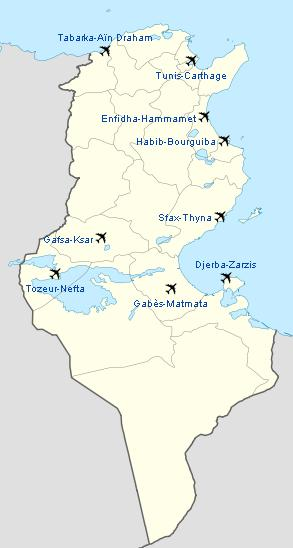
\includegraphics[width=6cm,height=8cm]{presentation/pres1.jpg}
\end{center}
%légende de l'image
\caption{Les divers aérodromes dans le FIR tunisien}
\end{figure}

L'office de l'aviation civile et des aéroports est chargé notamment des missions suivantes:\\
\begin{itemize}
\item L'exploitation, l'aménagement et le développement des aéroports ainsi que l'accomplissement de toutes les opérations et services nécessaires aux voyageurs, aux aéronefs, au fret et au courrier aérien dans les aéroports, \\
\item Le contrôle régional, la gestion de la navigation aérienne et la participation à l'exécution des plans de recherches et de sauvetages, \\
\item La délivrance de tous les documents requis pour le personnel aéronautique, les aéronefs et la navigation aérienne conformément à la législation en vigueur, \\
\item Accomplir la mission du contrôle de la navigation aérienne conformément aux normes internationales en assurant la sécurité, la régularité et la  Fluidité du trafic requis, \\
\item Maintenir aux plus hauts niveaux la sûreté et la sécurité des aéroports conformément aux dispositions internationales, \\
\item Veiller à l'adaptation des installations et des infrastructures aéroportuaires au besoin du trafic aérien, \\
\item Assurer la sécurité et la régularité du trafic en route dans les limites de l'espace aérien. \\
Pour faire à ces obligations internationales et assurer ses responsabilités dans le domaine de la sécurité aéronautique, un centre de navigation aérienne a été implanté par l'OACA. \\
\end{itemize}
\subsection{Organigramme de la Direction des Equipements de la Navigation Aérienne}

La direction des équipements de la navigation aérienne regroupe quatre divisions:\\
\begin{itemize}
\item Division Radar, \\
\item Division Etude et Coordination,\\
\item Division Equipements Aides à la Navigation Aérienne,\\
\item Division Télécommunication Aéronautique (Unité d’accueil).
\end{itemize}
\begin{figure}[!h]
\begin{center}
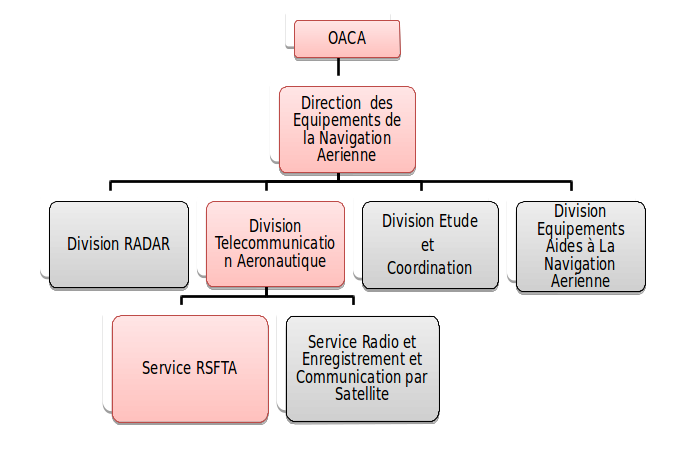
\includegraphics[width=15cm,height=6cm]{presentation/organisme.png}
\end{center}
\caption{Organigramme de la Direction des Equipements de la Navigation Aérienne}
\end{figure}
\subsection{Activités internationales}
Sur le plan international, l’Office de l’Aviation Civile et des Aéroports (OACA) occupe une place de plus en plus importante au sein des instances arabes, africaines et mondiales telles que le Conseil de l’Aviation Civile des Pays Arabes (A.C.A.C), la Commission Africaine de l’Aviation Civile (C.A.F.A.C), l’Organisation de l’Aviation Civile Internationale (O.A.C.I), le Conseil International des Aéroports (A.C.I)… \\

L’O.A.C.A est membre du Conseil International des Aéroports Région Afrique et préside le Groupe Régional de Planification et de Mise en Oeuvre de Plan de Navigation Aérienne pour l’Afrique et l’Océan Indien (A.P.I.R.G). Il est également membre du Conseil d’Administration du Fonds A.C.I.\\

L’Office s’est distingué ces dernières années par la qualité de l’organisation, en Tunisie, de manifestations et de conférences de taille se rapportant aux domaines de l’aviation civile, la gestion et la sûreté aéroportuaire.\\

L’O.A.C.A a également signé des conventions de partenariat avec son homologue au Maroc (O.N.D.A), la Société des Aéroports en Mauritanie (S.M.A), la Société des Aéroports de Paris (A.D.P) et l’Aéroport de Nice Côte d’Azur.\\

L'O.A.C.A emploie des compétences souvent sollicitées pour des travaux d’assistance et d’échange d’expérience avec d’autres pays de notre continent.\\

Les associations et les structures qui évoluent au sein de l’O.A.C.A, telles que l'Association Tunisienne des Contrôleurs de la Circulation Aérienne (A.T.C.C.A), l'Association des Electroniciens de la Sécurité Aérienne (A.T.E.N.A), l'Association des retraités de l'Office, l'amicale du personnel ainsi que l'Association Sportive (A.S.A.C.A), contribuent à renforcer le rayonnement de l'Office à l'échelle internationale par la participation de ces associations et structures à ce niveau à des activités diverses sportives, techniques, sociales….\\

\subsection{Service Réseau de Services Fixes de Télécommunications Aéronautiques}

Le service RSFTA  relève de la Direction des équipements de la navigation aérienne du Centre de Contrôle Régional. Elle  opère avec le Bureau Central des Télécommunications Aéronautiques qui est aussi le centre COM principal de Tunis et fonctionne en étroite collaboration avec le Service d’Information Aéronautique. Elle est chargée de la gestion, l’exploitation et la supervision du système autocommutateurs des messages aéronautiques (ADAMS) qui constitue une composante primordial du Réseau des services Fixes des Télécommunications Aéronautiques (RSFTA). \\

N’importe quel pays dont l'espace aérien sera traversé par le vol est dit pays partageant  ce vol et le besoin d'échange d'information entre pays qui partagent un vol est primordial.
Cet effort de collaboration fut possible pendant de nombreuses années grâce à l'aide de l’Aeronautical Fixed Telecommunications Network (AFTN) ou (RSFTA) en Français. \\
\section{Présentation du système autocommutateur des messages aéronautiques et du réseau AFTN/AMHS}

\subsection{Présentation du réseau AFTN (RSFTA)}

Le réseau des services fixes de télécommunications aéronautiques (RSFTA)  est un réseau mondial des circuits fixes aéronautiques, destiné dans le cadre du service fixe aéronautique, à l’échange des messages et/ou des données numériques entre les stations fixes aéronautiques ayant des caractéristiques de communications identiques ou compatibles. Ces messages aéronautiques ont essentiellement pour but d’assurer la régularité et la sécurité des vols  dans l’espace aérien tunisien. \\ 

Les différentes Catégories des messages qui sont  acheminées par le réseau du service fixe des télécommunications Aéronautiques sont : \\


\begin{itemize}
\item Messages de détresse. \\
\item Messages d’urgence. \\
\item Messages intéressant la sécurité et la régularité (plan de vols, autorisations de survole….). \\
\item Messages météorologiques (METAR, ….). \\
\item Messages des services d’informations aéronautiques (AIS:Notam, Snowtam,..). \\
\item Messages administratifs aéronautiques. \\
\item Messages de service. \\
\end{itemize}
Au niveau de chaque pays le réseau AFTN gère deux types de clients terminaux: \\

	\begin{itemize}
    \item \textbf{Clients nationaux:} Les différents aéroports nationaux et les différentes organisations de l’aviation civile locales ainsi que tout autre siège local pouvant échanger des messages aéronautiques. \\
    
    \item \textbf{Centres internationaux:} Ils sont formés par les centres adjacents qui constituent des nœuds du réseau AFTN et qui assure la fonction de relais pour la transmission des messages aéronautiques entre les différents pays du réseau mondial, dans le cas de la Tunisie les centres adjacents sont Rome, Alger, Tripoli et le Caire.\\

	\end{itemize}

La Tunisie est considérée comme un centre COM principal, parmi six centres principaux de l’Afrique. \\

\begin{figure}[!h]
\begin{center}
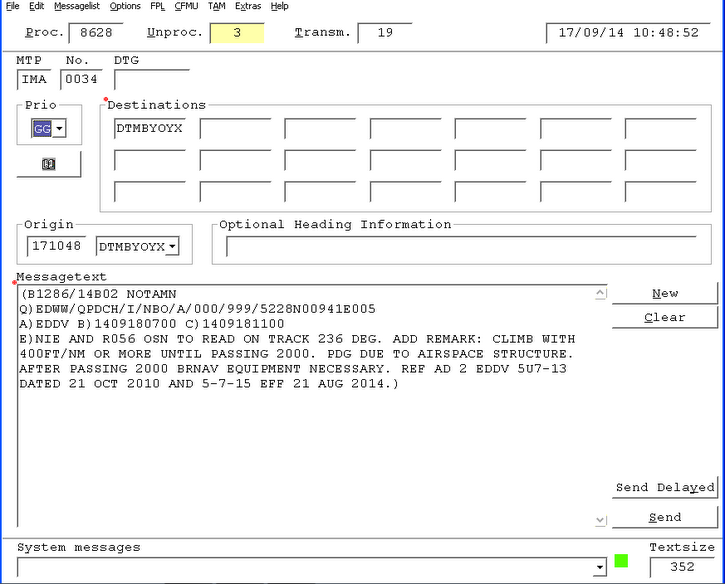
\includegraphics[width=14cm,height=8cm]{presentation/ftn.png}
\end{center}
%légende de l'image
\caption{Exemple de Message AFTN}
\end{figure}
Les champs d’un message AFTN se composent de:\\
\textbf{IMA 0034:} Identification de transmission\\
\textbf{GG:} Indicateur de priorité\\
\textbf{DTMBYOYX:} Indicateur de destinataire \\
\textbf{Origin 171048:} Moment du dépôt (Le groupe date-heure de 6 chiffres précisant le moment auquel le message a été déposé) \\
\textbf{DTMBYOYX:} Indicateur d’origine (identifiant l’expéditeur du message) \\
\textbf{Message Texte:} le contenu du message \\
\subsection{Présentation du Réseau AMHS}

Le réseau AMHS (ATS Message Handling System) est un standard pour la communication  aéronautique sol-sol.Il a été conçu pour remplacer le réseau actuel AFTN vu que ce dernier devenus de plus en plus lourds d’utilisation face à la multiplication importante et active du nombre des intervenants ainsi que l’augmentation considérable, en conséquence, des demandes associées aux services des télécommunications aéronautiques. En effet, en vue d’intégrer le futur réseau mondial de gestion des messages aéronautiques basé sur la technologie IP, pour cela la mise en œuvre de l’AMHS s’est avérée nécessaire. \\

L’avènement de ce nouveau réseau a permis entre autres : \\
\begin{itemize}
\item L’amélioration des services de télécommunications offerts par l’AFTN. \\
\item L’intégration d’autres protocoles de communication tels que le courrier électronique. \\ 
\item L’amélioration de la sécurité du réseau. \\
\item L’interopérabilité avec les autres services de messageries SITA, service militaire, bureau de piste…  \\
\item Le non limitation de longueur ou de type de message avec possibilité d’envoyer des pièces jointes (cartes aéronautiques). \\

\end{itemize}

\section{Présentation du projet}

Dans cette section, le projet sera mis dans son cadre général.\\

\subsection{Cadre du stage}
Ce stage d’immersion en entreprise s’inscrit dans le cadre de formation d’ingénieur en informatique à l’École Nationale des Sciences de l’Informatique (ENSI). Le présent travail se déroule au sein de l’entreprise OACA durant la période entre 01/08/2016 et 09/09/2016.
\subsection{Présentation du sujet}
Il s'agit de l’exécution d’une opération d’apurement pour remédier à la lenteur importante observée au niveau de la production des PIB ainsi que l’élaboration des check-lists. L’apurement des bases de données distantes situées au niveau des différents aéroports a pour objectif de faciliter le travail des exploitants. Notre tâche consiste alors à concevoir une solution pour l'apurement de la base de données de serveur de messages et la développer dans une application.\\
\section*{Conclusion}

Dans ce chapitre nous avons présenté l’entreprise accueillante ainsi que le projet à réaliser et son cadre. Dans le prochain chapitre nous détaillerons quelques concepts en relation avec le sujet afin de mieux
comprendre le déroulement de ce projet.


